\section{Discrete Fourier Transform}

\subsection{Theoretical aspects}
Often the \emph{discrete fourier transform} (\dft) is defined as an operation
acting on a $n$-tuple of complex numbers. In this project we opt to use a more
general and abtract formulation \cite{furer07}. For that purpose, instead of complex numbers we
will be refering to elements of an abstract algebraic ring $\Ring$, see appendix
\ref{app:ring} for a proper definition of ring. 
\begin{definition}
    The $n$-point \emph{discrete Fourier transform} is a linear
    automorphism of the $n$-tuples of $\Ring$ such that $(a_0,a_1,\ldots,a_{n-1})$
    is mapped into $(b_0,b_1,\ldots,b_{n-1})$ according to the formula 
    \begin{equation} 
        b_k = \sum_{j=0}^{n-1} w^{kj} a_j,
        \label{eq:dft}
    \end{equation}
    where $w$ is a principal \xroot{n}\ of unity.
    \label{def:dft}
\end{definition}
Note that the \dft\ depends on the choice of $w$.

For $w$, being an principal \xroot{n}\ of unity means that $w^k=1$ if and only if $n$
divides $k$. And from that we can prove that
\begin{equation}
    \sum_{j=0}^{n-1} w^{kj} = 
    \begin{cases} 
        n,\text{if $n$ divides $k$};\\ 
        0, \text{otherwise}.
    \end{cases}
\end{equation}
Also note that the multiplicative inverse is not guaranteed to exist for any
element of $\Ring$. Yet for $w$ a multiplicative inverse does exist, since
$w \cdot w^{n-1} =  w^{n-1} \cdot w = 1$, that is
\begin{equation}
    w^{-1} = w^{n-1}.
\end{equation}
With the properties of $w$, it is not difficult to check that the inverse of the
\dft\ (\ref{eq:dft}) is accomplished by performing a \dft\ using $w^{-1}$
instead of $w$ and taking into account and extra $\frac{1}{n}$ factor
\begin{equation} 
    n \cdot a_k = \sum_{j=0}^{n-1} (w^{-1})^{kj} b_j,
    \label{eq:inv_dft}
\end{equation}

\begin{example}
    When we deal with complex numbers $\Ring = \Complex$, an \xroot{n}\ of unity
    can be constructed as $w = \exp(- 2 \pi i/n)$, where $i = \sqrt{-1}$.
    Then the \dft\ takes the form
    \begin{equation} 
        b_k = \sum_{j=0}^{n-1} e^{-\frac{2\pi i}{n} kj}  a_j,
        \label{eq:complex}
    \end{equation}
    often used in signal processing and physics and called the \emph{forward} \dft.
    If we use instead $w^{-1} = \exp(2 \pi i/n)$ we are computing the
    \emph{backward} \dft.
    \label{ex:complex}
\end{example}

\begin{example}
   For a given prime number $p$, let $\Integer_p$ be the reduced residue system
   modulo $p$, ie. this set satisfies the ring axioms (in fact it is a finite
   field which is a sub-class), and let $g$ be a primitive root of $p$, ie. in the
   sense that the least non-zero value of $k$ for which $g^k \equiv 1 \pmod p$ is
   $k=p-1$. Then if $n$ divides $p-1$ we can construct $w = g^{(p-1)/n}$, which
   is an \xroot{n}\ of unity in $\Integer_p$. That said, the \dft\
   (\ref{eq:dft}) with $w = g^{(p-1)/n}$ is known as the \emph{Number-Theoretic
   Transform} (\ntt) which has applications such as the Sch\"onhage-Strassen
   algorithm for large integer number multiplication.
   \label{ex:ntt}
\end{example}

A brute force implementation of the \dft\ (\ref{eq:dft}) will involve
$\Order(n^2)$ multiplication and addition operations.
\emph{Fast Fourier Transform} (\fft) algorithms allow to compute the \dft\ with
lower complexity bounds, usually $\Order(n \log n)$.
The most famous \fft\ algorithm is known as Cooley-Tukey \cite{cooley65}, which
was proposed to compute \fft{}s only when $n$ is a power of two and has
assymptotical complexity $\Order(n \log_2 n)$.
Good-Thomas 
algorithm\footnote{\url{https://en.wikipedia.org/wiki/Prime-factor_FFT_algorithm}}
is a generalization of Cooley-Tukey's for any value of $n$, and it yields the
solution using $\Order(n (p_1 + p_2 + \ldots + p_k) )$ mutiplication and
addition operations where $p_1,\ldots,p_k$ is a prime sequence that factorizes $n = p_1\cdot
p_2 \ldots p_k$. 
Good-Thomas is a good candidate for a template \fft\ when the
underlying type satisfies the ring axioms and nothing more.
The problem with this algorithm is that the complexity is $\Order(n^2)$ for $n$
prime. For the particular case when underlying type corresponds to the complex numbers, 
$\Ring = \Complex$, 
Rader's \fft\ \cite{rader68}
can be used to compute the \dft\ in $\Order(n\log n)$ when $n$ is a prime
number. Again this algorithm can be templated on the type, since there may be
countless representations of real and complex numbers.

\subsection{Circular Discrete Convolution}
Rader's \fft\ algorithm takes advantange of the so-called
\emph{convolution theorem} in order to solve efficiently the \dft\ of prime size, 
and conversely having \fft\ capabilities allow
us to compute convolutions faster. Hence we regard as
inevitable to provide \dft\ and convolutions within the same library.
Here we will be discussing the \emph{Circular Discrete Convolution} (\cdc)
because it integrates seamlessly with the \dft\ on tuples of finite size.
\begin{definition}
    Given two $n$-tuples in the ring $\Ring$: 
    $a = (a_0,a_1,\ldots,a_{n-1})$ and $b=(b_0,b_1,\ldots,b_{n-1})$;
    the \emph{Circular Discrete Convolution} denoted as 
    $c = a\star b$ is another
    $n$-tuple such that
    \begin{equation} 
        c_k = \sum_{j=0}^{n-1} a_j \cdot b_{(k-j) \mod n}.
        \label{eq:convolution}
    \end{equation}
    \label{def:convolution}
\end{definition}
The \emph{Convolution Theorem} states that the \cdc\ of two $n$-tuples $a$ and
$b$ can be computed as follows
\begin{equation}
    c = \dft^{-1}\big( \dft(a) \cdot \dft(b)  \big),
    \label{eq:conv_theorem}
\end{equation}
where the dot operator for two $n$-tuples is understood as the element-wise
multiplication. This means that the \cdc\ of size $n$ can be computed with the
same computational complexity of the \dft, $\Order(n\log n)$ if the \fft\
algorithms are used instead of $\Order(n^2)$ if we use equation
(\ref{eq:convolution}) directly.

\subsection{Real transforms}\label{subsec:real}
Very often, the applications of Fourier methods involve the \dft\ in its complex
form (\ref{eq:complex}) where the input tuple $a = (a_0,a_1,\ldots,a_{n-1})$ are
real numbers.
The ouput tuple $b = (b_0,b_1,\ldots,b_{n-1})$ are complex numbers that satisfy
the following \emph{conjugate symmetry} 
\begin{equation}
    b_{k} = b^*_{n-k}.
    \label{eq:rfft_sym}
\end{equation}
This particular use case allows for an optimization in computation and memory of
a factor of 2. First of all, because the output has $n$ degrees of freedom as
the input; instead of $2n$ as it happens in general with $n$ unconstrained
complex numbers. Instead of returning $n$ complex numbers, some interfaces like
\fftw\ and \texttt{numpy}\footnote{\url{numpy.org}} return $\floor{n/2}+1$
complex numbers, thus discarding spurious values.

Formally, these type of transforms can be understood as a linear map from $\Real^n$ to the
space of the so called \emph{halfcomplex} numbers $\hComplex^n$, ie.
the subset of $\Complex^n$ that satisfy (\ref{eq:rfft_sym}).
One can prove that both backward and forward \dft\ acting on a halfcomplex array
$b$ yields $n$ real numbers, and the result of both the operations are related to
each other by an index inversion. That is, let $b\in \hComplex^n$ if 
$a = \dftf(b)$ and 
$a' =\dftb(b)$, then $a,a'\in \Real^n$ and $a_k = a'_{n-k}$.
Also, it can be show that for any $a\in\Real^n$ if $b=\dftf(a)$ then
$b\in\hComplex^n$ and $b^* = \dftb(a)$, where $b^*\in\hComplex^n$ is the complex
conjugate of $b$.
Figure \ref{fig:halfcomplex}
represents the 4 node graph obtained by repeated application of forward and
backward \dft\ in $\Real^n$ or $\hComplex^n$ to summarize the previous
description.
\begin{figure}
    \centering
    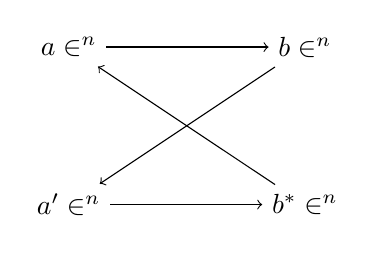
\begin{tikzpicture}
    \node (a1) at (0,-2) {$a \in \Real^n$};
    \node (a2) at (0,-4) {$a' \in \Real^n$};
    \node (b1) at (3,-2) {$b \in \hComplex^n$};
    \node (b2) at (3,-4) {$b^* \in \hComplex^n$};
    \path[->] (a1) edge (b1) ;
    \path[->] (a2) edge (b2) ;
    \path[->] (b1) edge (a2) ;
    \path[->] (b2) edge (a1) ;
    \end{tikzpicture}
    \caption{Real vectors (on the left) under \dft\ transformations yield
    halfcomplex (on the right),
    while halfcomplex yield real. The arrows indicate the result of the forward
    \dft, the backward \dft's are found by inverting the arrows. Vector $b^*$ is
    the complex conjugate of $b$ and $a'$ is related to $a$ by index inversion.}
    \label{fig:halfcomplex}
\end{figure}

There are countless of ways to represent vectors of $\hComplex^n$.
In our \api\ we use a tuple of $n$ real numbers
\[ 
    (r_0,r_1,r_2,\ldots,r_{ \floor{n/2} },i_{\floor{n/2}+1},\ldots,i_{n-2},i_{n-1})
\]
where $r_k = \real(b_k)$ and $i_k = \imag(b_k)$.

% 
% The first point above makes me think that at this point we should have
% separate classes to handle two types of transform philosophy: complex dft and
% ring dft. Moving forward with this proposal will break the nice symmetry that
% we previously have where ring transforms were handle as if they were complex,
% with the underlying static type selection making all the work to select the
% appropriate algorithms. On the bright side having these two api's will give
% the user more control of what is being done and we no longer need is_complex
% to select appropriate algorithms. Notice that ring transforms can also apply
% to complex numbers, with the appropriate selection of the root of unity, this
% is why I thought they might be unified at first.
% 
% If we introduce real-to-complex into the game, we could either expand the
% complex dft class to accommodate this case or we could introduce a third class
% specific to it. In any case I think we are likely bound to have template
% parameters specifying the Real and the Complex types, maybe having by default
% the following rule Real = Complex::value_type.

\subsection{\fftw}
\fftw\ \cite{FFTW05} is the \emph{de facto} library for computing \dft\ in the scientific
community for its wide problem domain and performance.
\fftw\ mixes different \fft\ algorithms and manages to achieve the computational
complexity of $\Order(n \log n)$ for any $n$-sized \dft. It does also
$D$-dimensional transforms and it is able to exploit multi-processor hardware by
either multi-threading or \mpi\ parallelizations. This library is highly portable
and yet it is competitive in performance with hardware specific codes such as
Intel's \emph{MKL}. One reason for the success of \fftw\ is its strategy to
generate fixed size \fft\ routines at compile-time for $1\le n\le 64$ called \emph{codelets}.
\dft{}s of a bigger size can be decomposed in smaller \dft{}s until the problem
fits into one such codelets.

Unfortunately, \fftw\ does not provide a C++ interface.
Hence the user is constrained to 
\begin{itemize}
    \item use raw pointers to communicate with its interface;
    \item \verb|reinterpret_cast<>| from
    \verb|std::complex<double>*| to \verb|fftw_complex*| when passing input/ouput
    pointers to its routines;
    \item disregard \verb|const| qualification for input pointers;
    \item produce \raii\ wrappers for \fftw's resources (such as
    \verb|fftw_plan|s and memory allocation) or risk to have exception unsafe
    code and leaks.
\end{itemize}
In addition to these technical issues that can eventually be circumvented with
the use of a wrapper\footnote{for example \url{github.com/dealias/fftwpp}},
\fftw\ was designed to compute \dft\ for
complex numbers, like in Example \ref{ex:complex}. 
There is no support for \dft{}s in the broader sense of Definition \ref{def:dft}.
For example, we cannot use \fftw\ to compute the \ntt{}s described in the
Example \ref{ex:ntt}. Also \dft\ can be computed for a limited number of real
number representation types: \verb|float|, \verb|double|, \verb|long double|
and the nonstandard \verb|__float128|.

There is another issue worth mentioning, which is that of the scalability of the
parallel \mpi\ routines for computing $3$-dimensional \dft. As it pointed out in
\cite{springel_2020,adamek_2016,pippig_13}, \fftw's approach to
$D$-dimensional
\dft\ consists in the
decomposition of the problem domain along one dimension, having as a consequence that
the number $P$ of partecipating \mpi\ processes can grow up to $n$, the side length
of the domain hypercube, while the memory requirement of the problem grows as
$\Order(n^D)$. Furthermore, the communication pattern to perform that operation
is \emph{all-to-all} meaning that every \mpi\ process must reach every other
$\Order(P)$ process for exchange of information.
Better domain decomposition strategies
exist though. The $D$-dimensional grid can be decomposed along $D-1$ dimensions
alleviating to a great extent the memory scalability problem---$P$ can grow up
to $n^{D-1}$ in this scheme---and for which
$\Order((D-1)\cdot P^{1/(D-1)})$ communications are required per process to
complete the \dft. For instance \cite{adamek_2016} uses a \emph{home-made}
3-dimensional \mpi\ \fft\ algorithm with 2-dimensional domain decomposition.
Roughly speaking, $P$ processes are arranged into a 2-dimensional grid of side
$\sqrt{P}$ and $\Order(\sqrt{P})$ \mpi\ communications are required per
process in order to perform one \dft. \cite{pippig_13} generalizes this
algorithm for $D$-dimensions.
